\documentclass[../main.tex]{subfiles}
\begin{document}
\paragraph{Offline solutions}\label{par:conservation_fom}

The FOM is assembled using the usual aglorithm of spatial semi-discretisation of the RHS of \eqref{eq:conservation} and subsequently using an Euler implicit time-stepping scheme to generate the desired snapshots

\begin{figure}[H]
    \centering 
    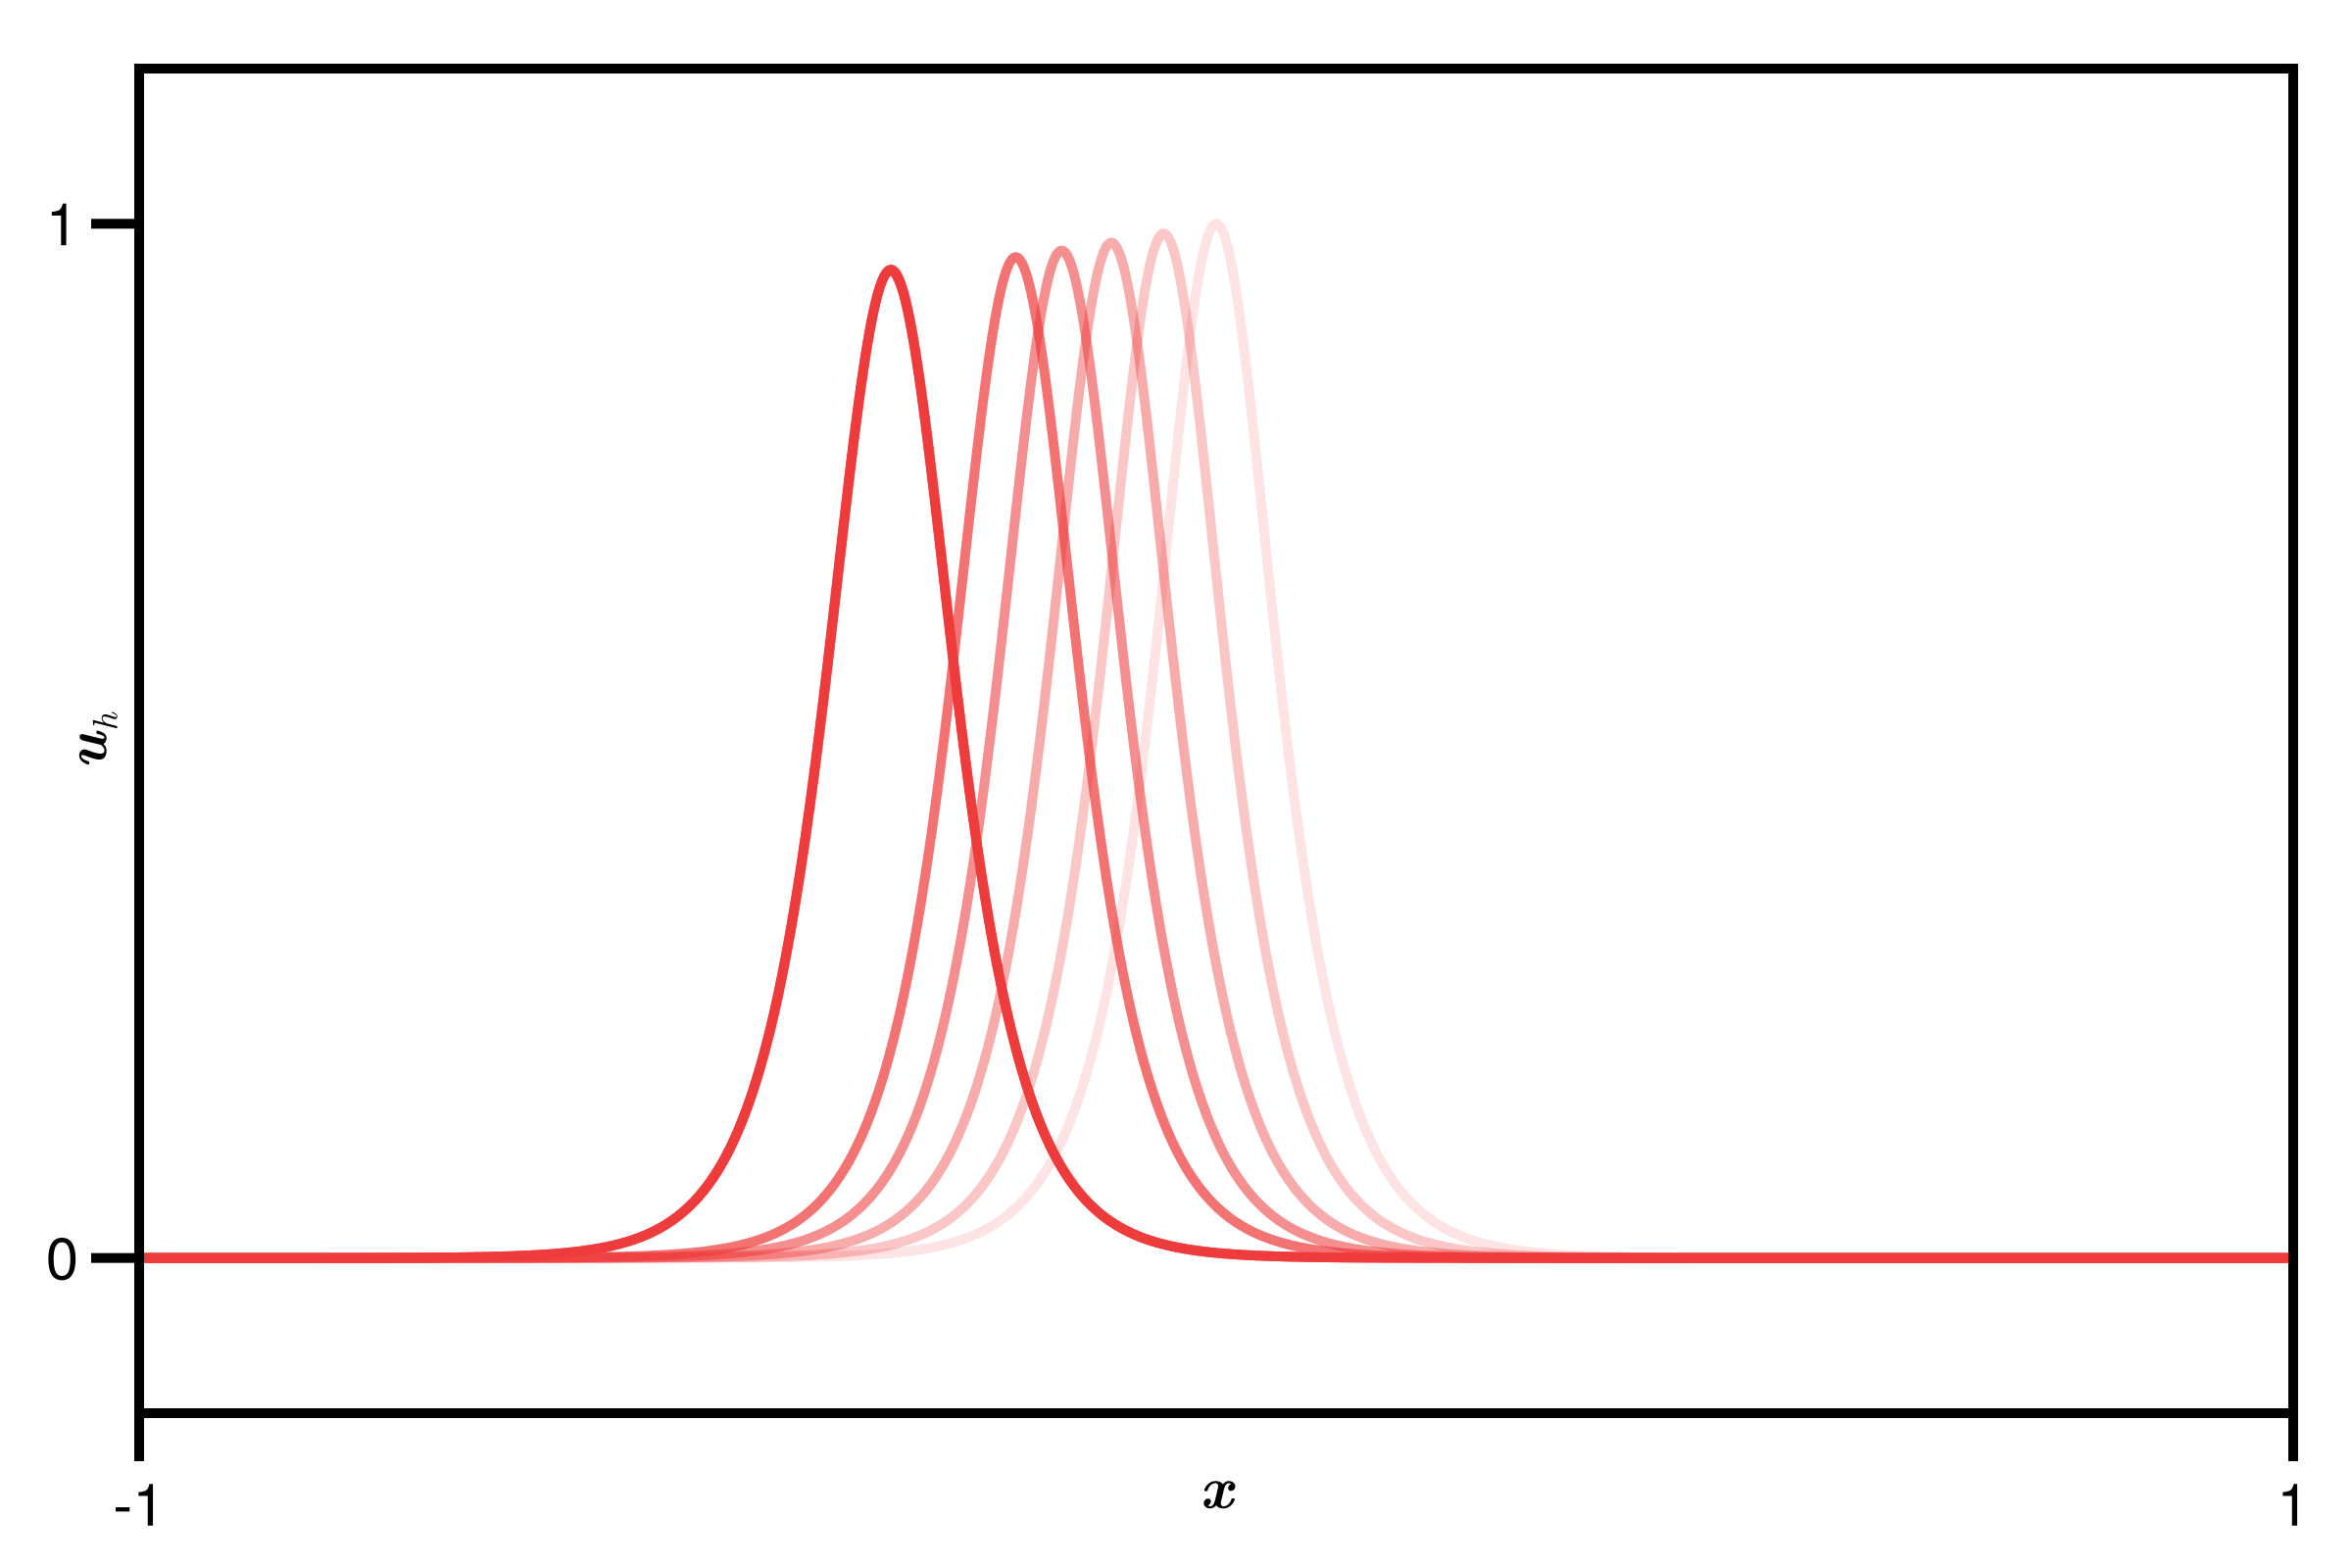
\includegraphics[keepaspectratio, width=0.7\textwidth]{../figures/fig:conservation_fom.png}
    \caption{Transient solutions of \eqref{eq:conservation} at full-order (lighter colors indicate older timesteps).}
    \label{fig:conservation_fom}
\end{figure}

\end{document}
